
\begin{center}
\Huge
Regressioner og regressionsanalyse
\end{center}
\section*{Regression}
\stepcounter{section}
Vi skal i dag se på regressionsanalyse.

\begin{exa}
Har vi et datasæt 
\begin{center}
\begin{tabular}{c|c|c|c|c|c|c|c|c|c|c}
$x$ & 1 & 2 & 3 & 4 & 5 & 6 & 7 & 8 & 9 & 10 \\ \hline
$y$ & 0.1 & 1 & 2 & 3.1 & 3.9 & 4.9 & 6.2 & 8.0 & 10.1 & 12.0
\end{tabular}
\end{center}
uden at vide, hvilken underlæggende sammenhæng, der skaber dataet, kan vi prøve at lave forskellige regressioner på det. Dette gøres i Maple og kan ses af Fig. \ref{fig:regression}

\begin{figure}[H]
\centering
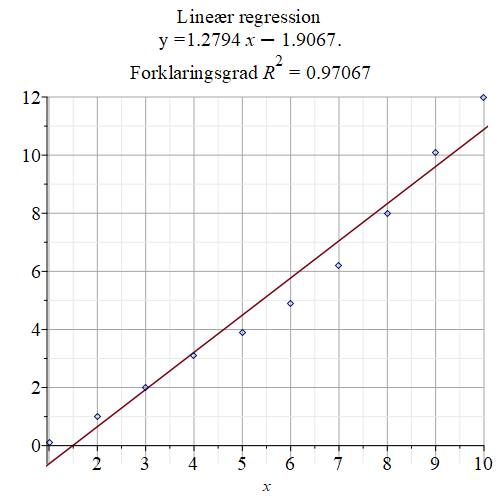
\includegraphics[width = \textwidth*4/10]{Billeder/linreg.png}
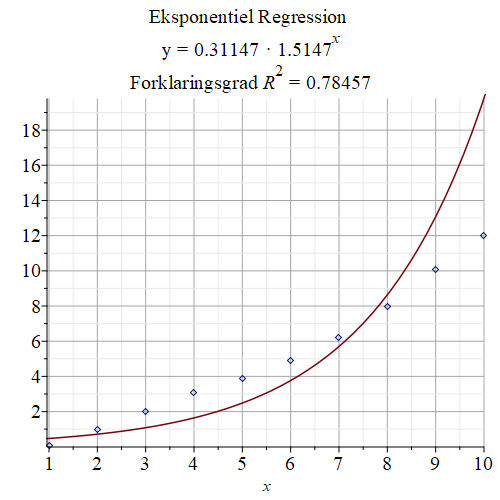
\includegraphics[width = \textwidth*4/10]{Billeder/expreg3.png}
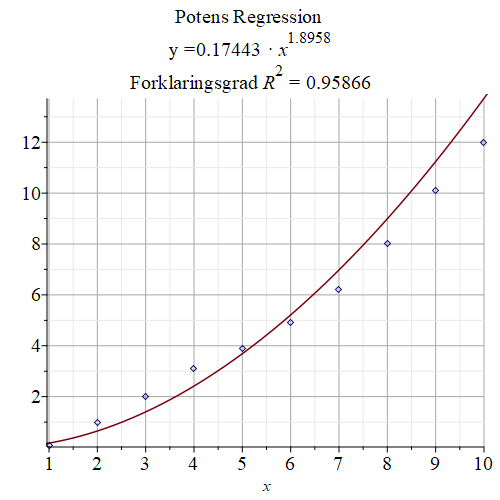
\includegraphics[width = \textwidth*4/10]{Billeder/powreg.png}
\caption{Lineær regression, eksponentiel regression og potensregression på datasæt}
\label{fig:regression}
\end{figure}
Hvordan afgør vi så, hvilken af modellerne der er bedst, hvis vi ikke har yderligere information omkring kilden af dataet? Man kan ikke sammenligne korrelationskoefficienter mellem modeller. Derfor skal vi lave regressionsanalyse. En del af regressionsanalyse er blot at betragte de fittede modeller og se, hvilken model der ser ud til at passe bedst. I dette tilfælde er det den lineære model eller potensmodellen. 
\end{exa}


\section*{Regressionsanalyse}

Til at vurdere, om en regression er god, skal vi bruge et værktøj til at afgøre, om det modellen rammer forbi blot er tilfældige fejl eller om vi rammer strukturelt forkert. Første tilfælde er ønskværdigt. Vi definerer nu residualerne til en regression.
\begin{defn}
Givet måledata $(x_1,y_1),(x_2,y_2),\hdots,(x_n,y_n)$ og regressionsmodel $f(x)$, så definerer vi det $i$'te residual som det, modellen $f$ rammer forbi den målte værdi. Mere præcist
\begin{align*}
r_i = y_i - f(x_i).
\end{align*} 
\end{defn}
Det er klart, at en god model $f(x)$ vil have små residualer. Udover dette så vil vi også have normalfordelte residualer. Det vil sige, at vi gerne vil have mange residualer tæt på 0 og kun få langt fra 0. Der må ikke være nogen yderligere struktur i residualerne. For at se, hvad dette betyder, ser vi på et eksempel.

\begin{exa}
Betragter vi regressionerne fra tidligere eksempel, kan vi finde residualerne for de tre modeller. Disse findes i Maple ved eksempelvis \texttt{plotResidualer(X,Y,LinReg)} i fald residualerne skal findes for lineær regression. Residualerne for de tre modeller kan ses af Fig. \ref{fig:resplot}
\begin{figure}[H]
\centering
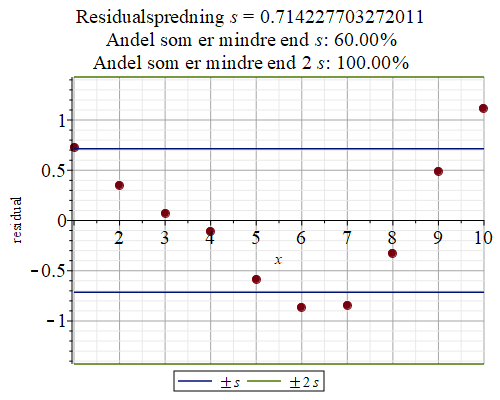
\includegraphics[width = \textwidth*4/10]{Billeder/residuallin.png}
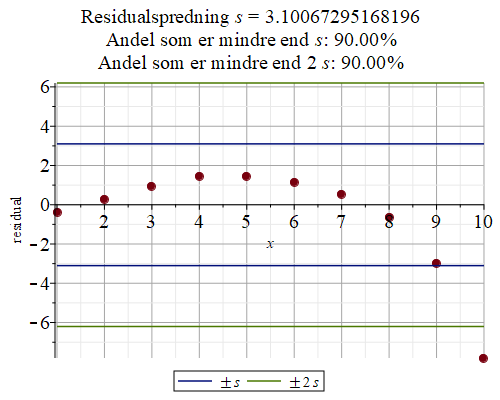
\includegraphics[width = \textwidth*4/10]{Billeder/residualexp.png}
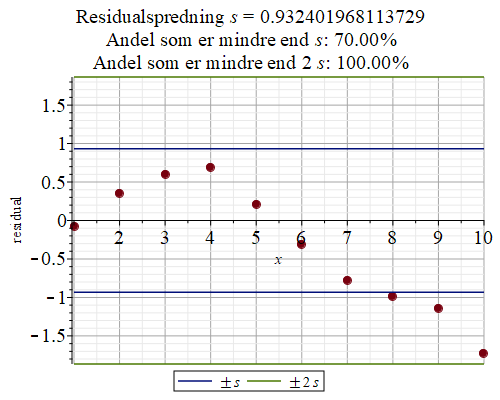
\includegraphics[width = \textwidth*4/10]{Billeder/residualpow.png}
\caption{Lineær regression, eksponentiel regression og potensregression på datasæt}
\label{fig:resplot}
\end{figure}
Det er lineær regression og potensregression, der har mindst spredning i residualerne, men det ser ud til, at der er struktur i residualerne for alle tre tilfælde. Derfor kunne det tyde på, at ingen af de tre regressioner passer godt til datasættet.
\end{exa}
\section*{Opgave 1}
\stepcounter{section}

Lav regression på følgende datasæt og afgør med residualanalyse hvilken model der passer bedst.
\begin{center}
\begin{tabular}{c|c|c|c|c|c|c|c|c|c}
1 & 2 & 3 & 4 & 5 & 6 & 7 & 8 & 9 & 10\\ \hline
1.45 & 14.96 & 7.22 & 26.63 & 45.49 & 66.88 & 103.90&157.63 & 162.63 & 252.61
\end{tabular}
\end{center}
Fjern efterfølgende sidste punkt og lav regression på de første 9 punkter. Se nu, hvilken model der rammer det sidste punkt bedst


\section*{Opgave 2}
Lav regression på følgende datasæt og afgør med residualanalyse hvilken model der passer bedst.
\begin{center}
\begin{tabular}{c|c|c|c|c|c|c|c|c|c}
1 & 2 & 3 & 4 & 5 & 6 & 7 & 8 & 9 & 10\\ \hline
1.22& 8.57 &12.73& 44.57&
 462.63& 66.85& 2620.83 &1765.227
& 2908.03& 5299.46
\end{tabular}
\end{center}
Fjern efterfølgende sidste punkt og lav regression på de første 9 punkter. Se nu, hvilken model der rammer det sidste punkt bedst


\section*{Opgave 3}
Lav regression på følgende datasæt og afgør med residualanalyse hvilken model der passer bedst.
\begin{center}
\begin{tabular}{c|c|c|c|c|c|c|c|c|c}
1 & 2 & 3 & 4 & 5 & 6 & 7 & 8 & 9 & 10\\ \hline
13.42& 17.81& 23.01& 18.37& 28.61& 35.09&
 36.54 &37.31& 48.88& 52.75
\end{tabular}
\end{center}
Fjern efterfølgende sidste punkt og lav regression på de første 9 punkter. Se nu, hvilken model der rammer det sidste punkt bedst
